\chapter{牛顿定律}
\section{作业习题}
\subsection*{一、填空题}
\begin{enumerate}
    \item 沿水平方向的外力$F$将物体$A$压在竖直墙上,由于物体与墙之间有摩擦力,此时物体保持静止,并设其所受静摩擦力为$f_0$,若外力增至$2F$,则此时物体所受静摩擦力为\nl。
    \item 如图 \ref{fig:3} ,在升降机天花板上拴有轻绳,其下端系一重物,当升降机以加速度$a_1$上升时,绳中的张力正好等于绳子所能承受的最大张力的一半,问升降机以多大加速度$a=\nl$上升时,绳子刚好被拉断。
    \begin{figure}[H]
        \centering
        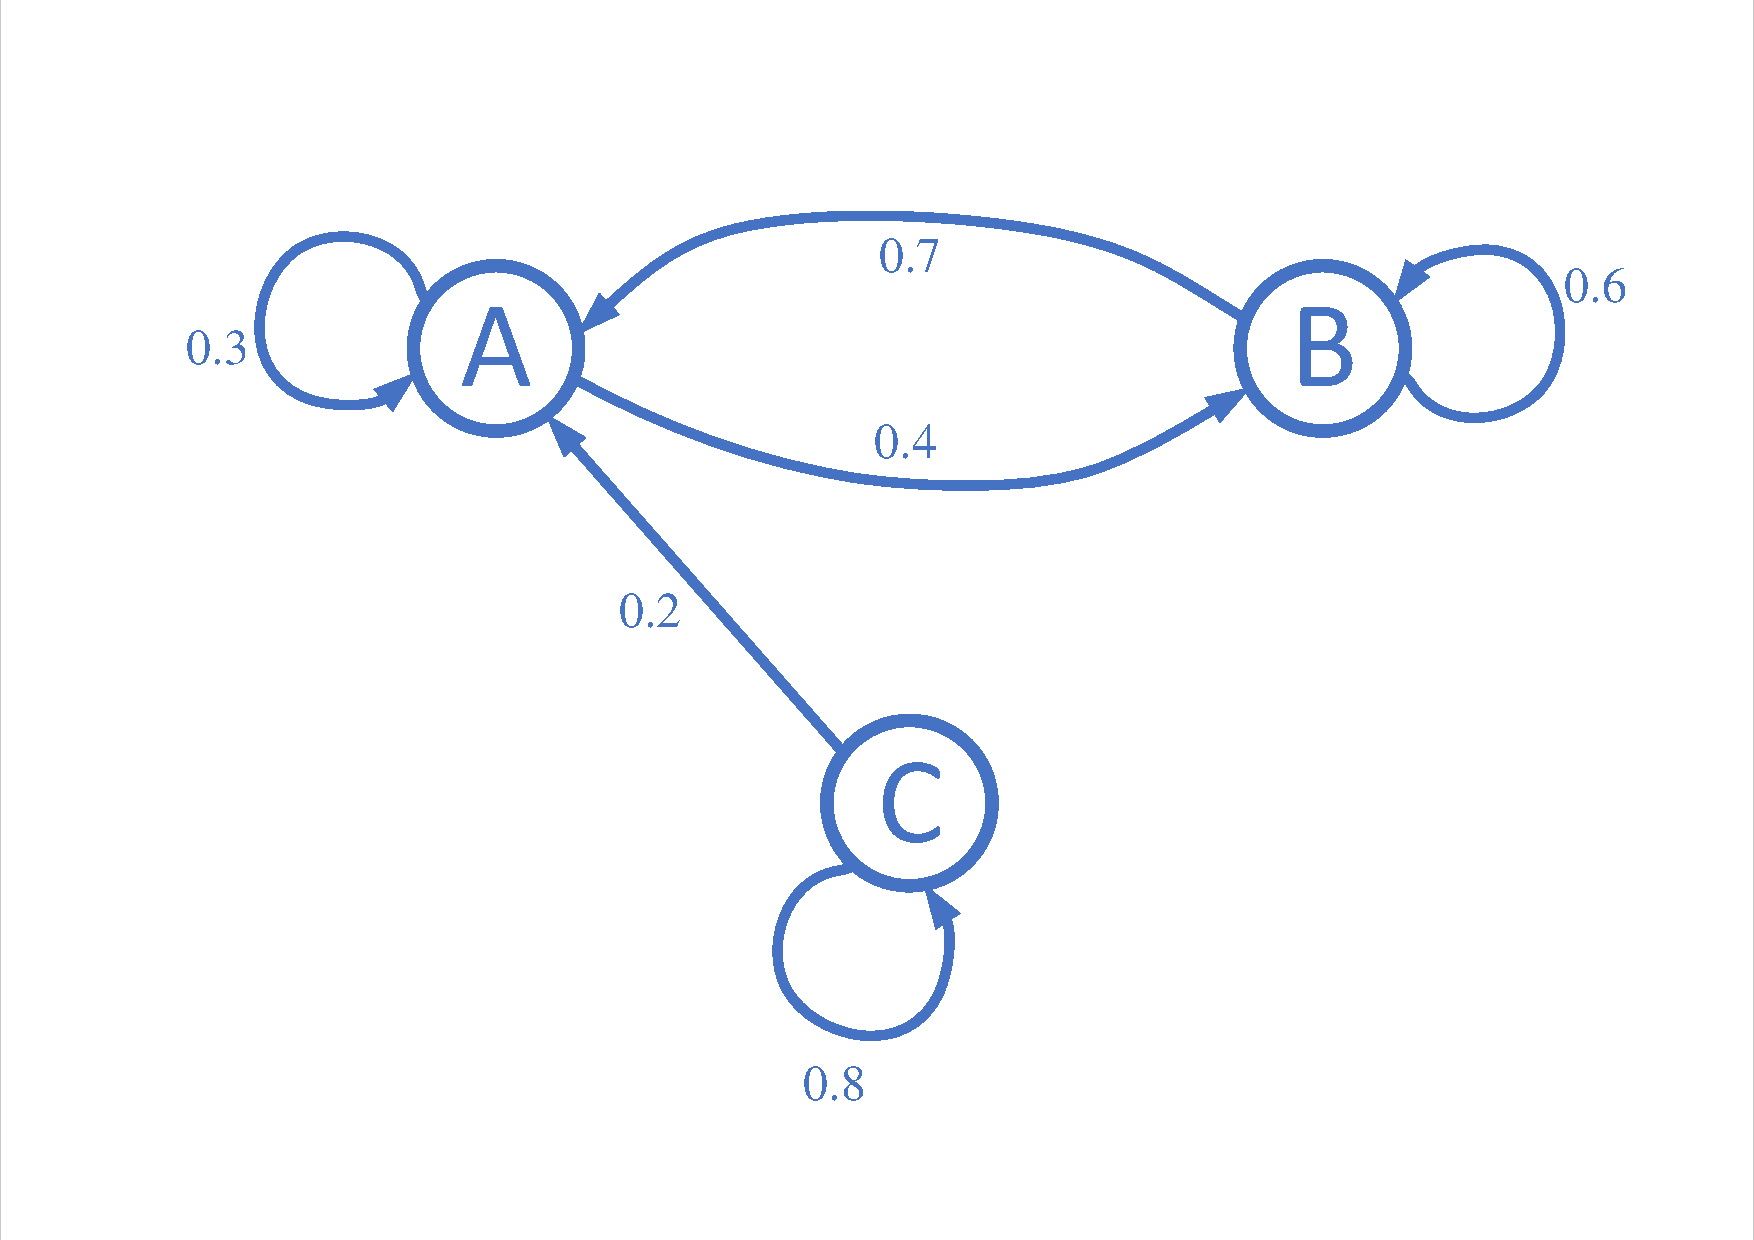
\includegraphics[width=0.15\textheight]{fig3}
        \caption{如图}\label{fig:3}
    \end{figure}
    \item 如图 \ref{fig:4} 一物体质量为$M$,置于光滑水平地板上.今用一水平力$\vec{F}$通过一质量为$m$的绳拉动物体前进,则物体的加速度$a=\nl$.  
    \begin{figure}[H]
        \centering
        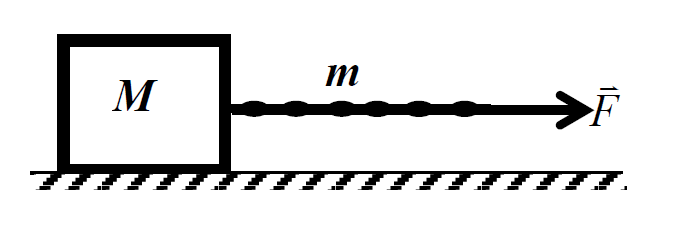
\includegraphics[width=0.15\textheight]{fig4}
        \caption{如图}\label{fig:4}
    \end{figure}
    \item 质量$\centering
    m=40 kg$的箱子放在卡车的车厢底板上,已知箱子与底板之间的静摩擦系数为$\mu_s=0.40$,滑动摩擦系数为$\mu_k=0.25$,当卡车以$a = 2 m/s^2$的加速度行驶时,作用在箱子上的摩擦力的大小$f =\nl $.                   
    \item 在如图所示 \ref{fig:5} 的装置中,两个定滑轮与绳的质量以及滑轮与其轴之间的摩擦都可忽略不计,绳子不可伸长,$m_1$与平面之间的摩擦也可不计,在水平外力$F$的作用下,物体$m_1$与$m_2$的加速度$a=\nl$.
    \begin{figure}[H]
        \centering
        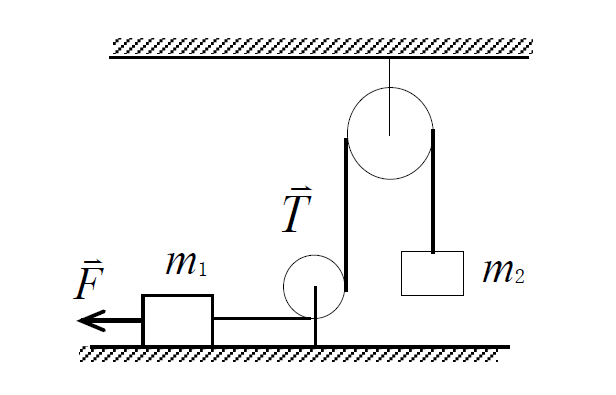
\includegraphics[width=0.15\textheight]{fig5}
        \caption{如图}\label{fig:5}
    \end{figure}

\end{enumerate}

\subsection*{二、选择题}
\begin{enumerate}
\item 如图 \ref{fig:6} , 在$m_A>μm_B$的条件下,可算出$m_B$向右运动的加速度$a$,今如取去$m_A$而代之以拉力$T=m_Ag$,算出的加速度$a′$则有: (\hspace{1pc})
\twoch{$a>a^{'}$ }{$a=a^{'}$ }{$a<a^{'}$ }{不能确定}
    \begin{figure}[H]
        \centering
        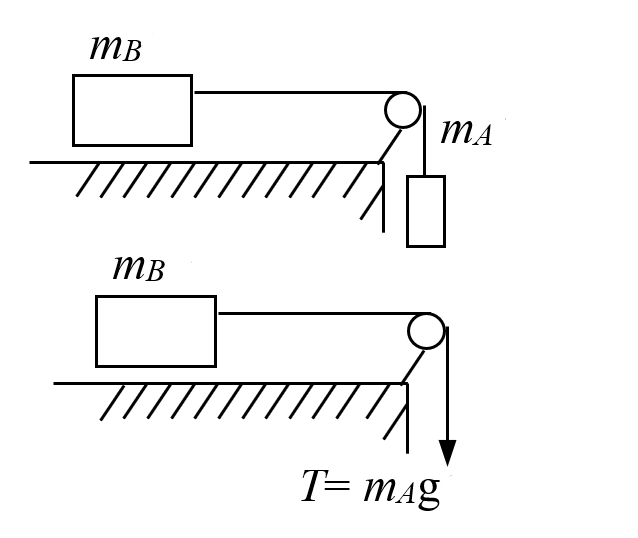
\includegraphics[width=0.15\textheight]{fig6}
        \caption{如图}\label{fig:6}
    \end{figure}
\item 如图\ref{fig:7} , $m$与$M$,$M$与水平桌面间都是光滑接触,为维持$m$与$M$相对静止,则推动$M$的水平力$F$为(\hspace{1pc})
\twoch{$(m+M)g\mathrm{cot}\theta$}{$(m+M)g\mathrm{tan}\theta$}{$mg\mathrm{tan}\theta$}{$Mg\mathrm{tan}\theta$}.
    \begin{figure}[H]
        \centering
        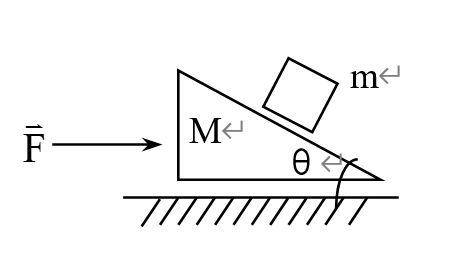
\includegraphics[width=0.15\textheight]{fig7}
        \caption{如图}\label{fig:7}
    \end{figure}
\item 一质量为$m$的质点,自半径为$R$的光滑半球形碗口由静止下滑,质点在碗内某处的速率为$V$,则质点对该处的压力数值为(\hspace{1pc})
\twoch{$\frac{mV^2}{R}$}{$\frac{3Mv^2}{2R}$}{$\frac{2mV^2}{R}$}{$\frac{5mV^2}{2R}$}
\item 如图 \ref{fig:8} ,滑轮、绳子质量及运动中的摩擦阻力都忽略不计,物体$A$的质量$m_1$大于物体B的质量$m_2$.在$A$、$B$运动过程中弹簧秤$S$的读数是(\hspace{1pc})
\twoch{$(m_1+m_2)g$}{$(m_1-m_2)g$}{$\frac{2m_1m_2}{m_1+m_2}g$}{$\frac{4m_1m_2}{m_1+m_2}g$}
    \begin{figure}[H]
        \centering
        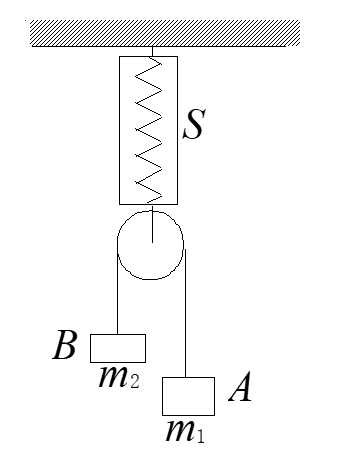
\includegraphics[width=0.15\textheight]{fig8}
        \caption{如图}\label{fig:8}
    \end{figure}

\item 如图所示 \ref{fig:9},质量为$m$的物体$A$用平行于斜面的细线连结置于光滑的斜面上,若斜面向左方作加速运动,当物体开始脱离斜面时,它的加速度的大小为:
\twoch{$g\mathrm{sin}\theta$}{$g\mathrm{cos}\theta$}{$g\mathrm{cot}\theta$}{$g\mathrm{tan}\theta$}
    \begin{figure}[H]
        \centering
        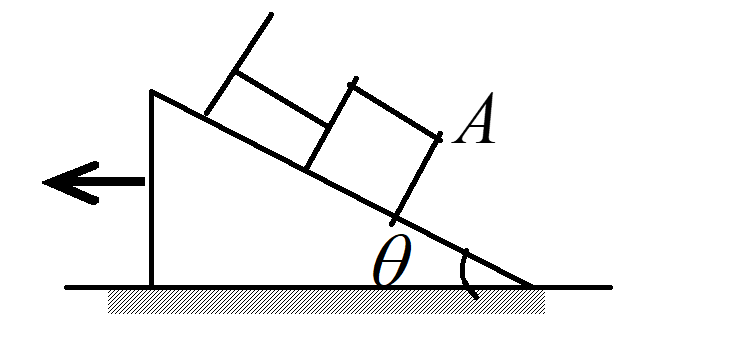
\includegraphics[width=0.15\textheight]{fig9}
        \caption{如图}\label{fig:9}
    \end{figure}
\item 站在电梯内的一个人,看到用细线连结的质量不同的两个物体跨过电梯内的一个无摩擦的定滑轮而处于“平衡”状态.由此,他断定电梯作加速运动, 
其加速度为(\hspace{1pc})
\twoch{大小为$g$, 方向向上}{大小为$g$, 方向向下}{大小为$\frac{1}{2}g$,方向向上}{大小为$\frac{1}{2}g$, 方向向下}
\end{enumerate}


\subsection*{三、计算题}
\begin{enumerate}
    \item 如图 \ref{fig:10} , 已知$m_A=2kg, m_B=1kg, m_A, m_B$与桌面间的摩擦系数$\mu=0.5(g=10m/s^2)$
    \begin{enumerate}
    \item[(1)] 今用水平力$F=10N$推$m_B$, 求$m_A$与$m_B$的摩擦力$f$及$m_A$的加速度$a_A$ ;
    \item[(2)] 今用水平力$F=20N$推$m_B$, 求$m_A$与$m_B$的摩擦力$f$及$m_A$的加速度$a_A$ .
        \begin{figure}[H]
            \centering
            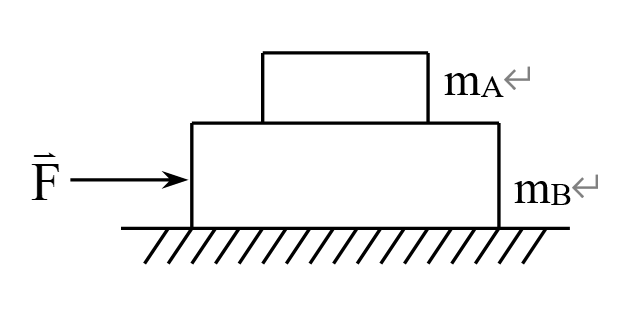
\includegraphics[width=0.15\textheight]{fig10}
            \caption{如图}\label{fig:10}
        \end{figure}
    \end{enumerate}
    \item 如图 \ref{fig:11} , 光滑水平面上平放着半径为$R$的固定环,环内的一物体以速率$V_0$开始沿环内侧逆时针方向运动,物体与环内侧的摩擦系数为$\mu$, 求:
    \begin{enumerate}
        \item[(1)] 物体任一时刻$t$的速率$V$;                                            
        \item[(2)] 物体从开始运动经$t$秒经历的路程$S$.
        \begin{figure}[H]
            \centering
            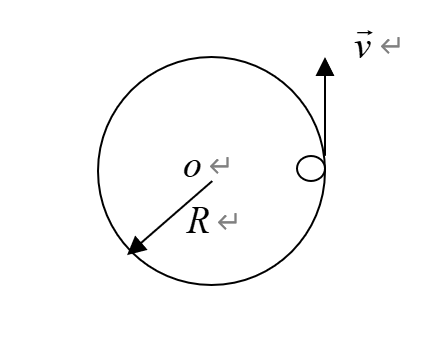
\includegraphics[width=0.15\textheight]{fig11}
            \caption{如图}\label{fig:11}
        \end{figure} 
    \end{enumerate}
\end{enumerate}

\section{习题参考答案}
\subsection*{一、填空题}
\begin{enumerate}
    \item 沿水平方向的外力$F$将物体$A$压在竖直墙上,由于物体与墙之间有摩擦力,此时物体保持静止,并设其所受静摩擦力为$f_0$,若外力增至$2F$,则此时物体所受静摩擦力为\anl{$f_0$}。
    \item 如图 \ref{Fig:3} ,在升降机天花板上拴有轻绳,其下端系一重物,当升降机以加速度$a_1$上升时,绳中的张力正好等于绳子所能承受的最大张力的一半,问升降机以多大加速度$a=\anl{$g+2a_1$}$上升时,绳子刚好被拉断。
    
    \begin{note}
        \\
       \textcolor{red} 
        {$\frac{F_{max}}{2}-mg=ma_1 \Longrightarrow F_{max} = 2mg(g+a_1) \Longrightarrow F_{max}-mg = ma \Longrightarrow a = g+2a_1$}
    \end{note}
    \begin{figure}[H]
        \centering
        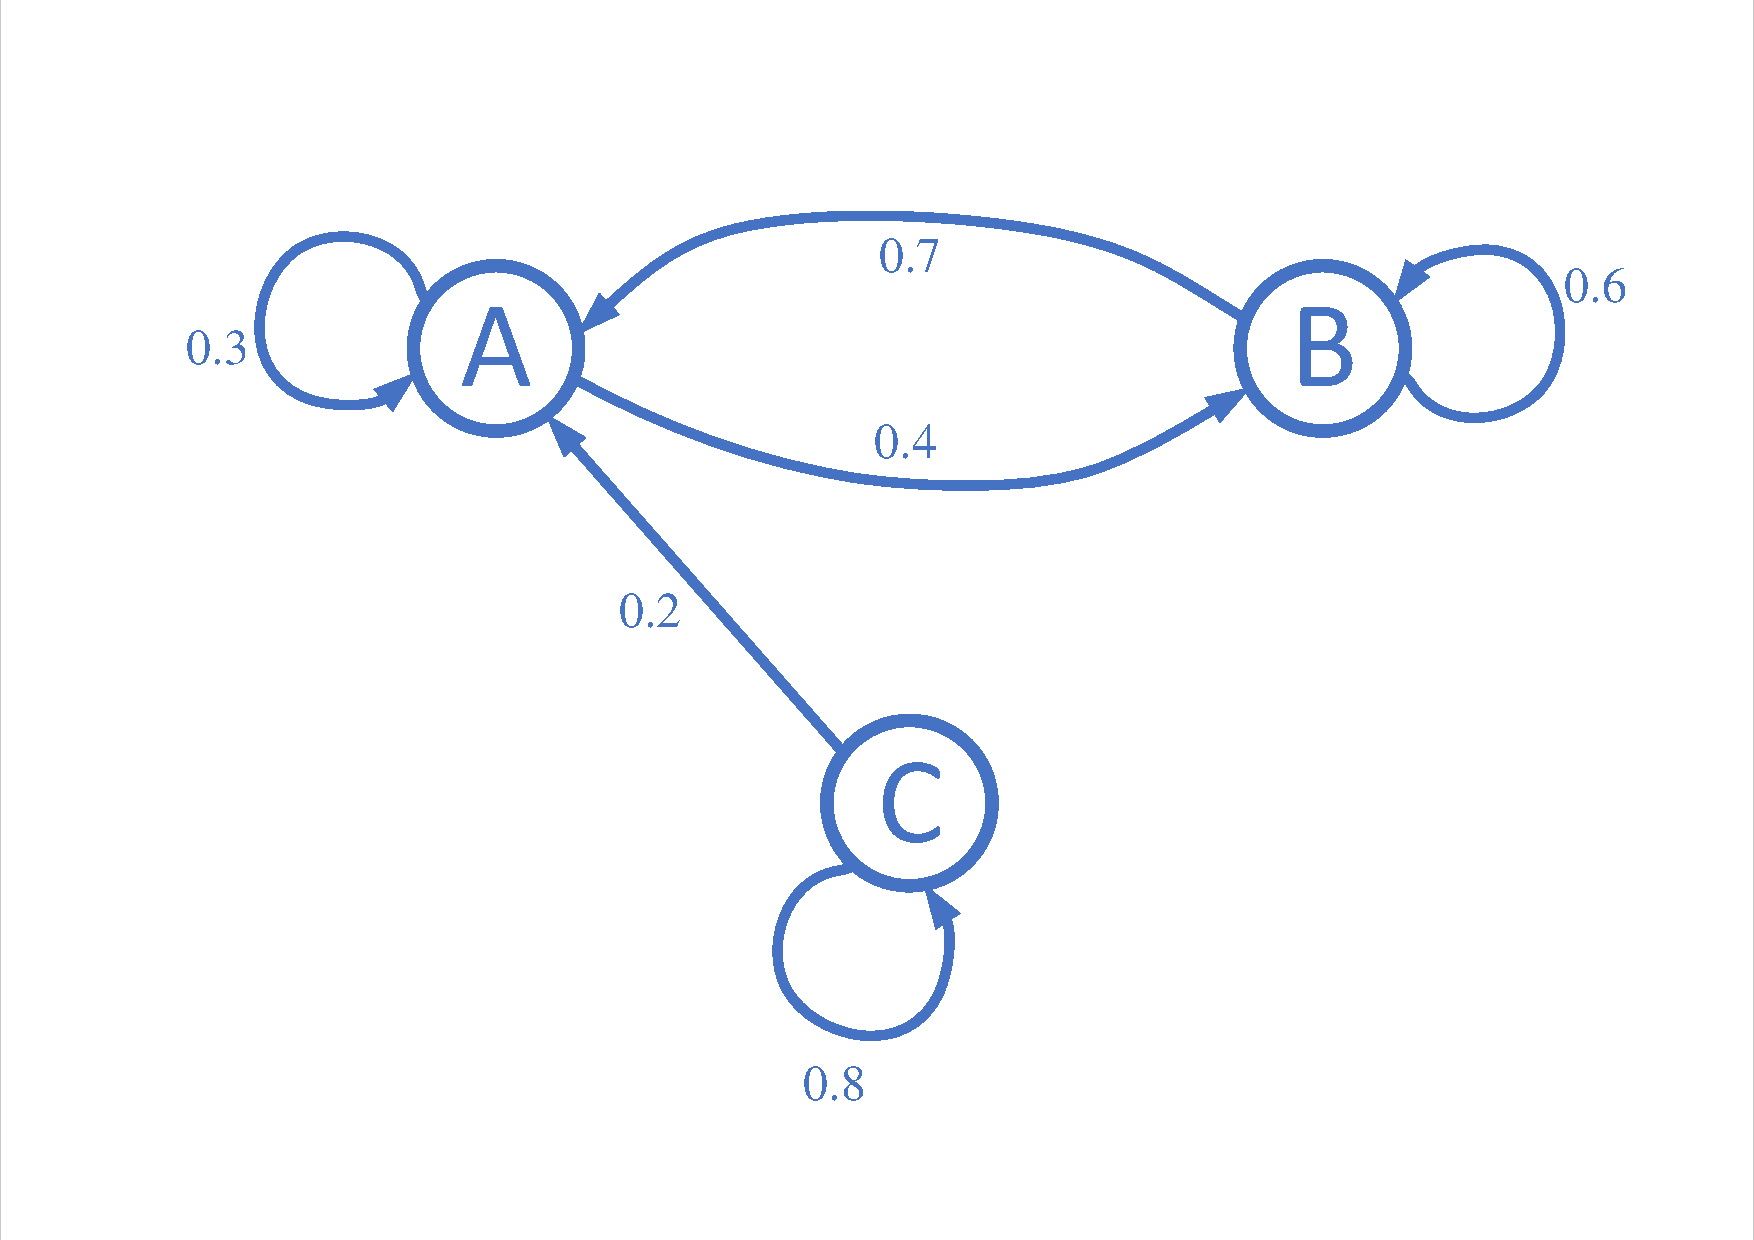
\includegraphics[width=0.15\textheight]{fig3}
        \caption{如图}\label{Fig:3}
    \end{figure}
    \item 如图 \ref{Fig:4} 一物体质量为$M$,置于光滑水平地板上.今用一水平力$\vec{F}$通过一质量为$m$的绳拉动物体前进,则物体的加速度$a=\anl{$\frac{F}{M+m}$}$.  
    \begin{figure}[H]
        \centering
        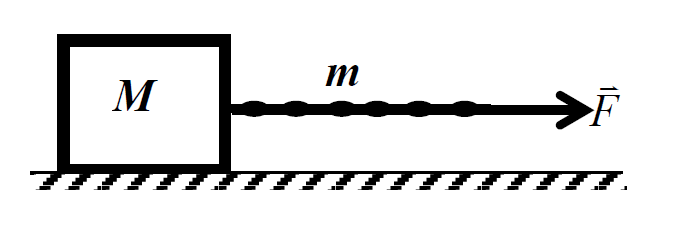
\includegraphics[width=0.15\textheight]{fig4}
        \caption{如图}\label{Fig:4}
    \end{figure}
    \item 质量$m=40 kg$的箱子放在卡车的车厢底板上,已知箱子与底板之间的静摩擦系数为$\mu_s=0.40$,滑动摩擦系数为$\mu_k=0.25$,当卡车以$a = 2 m/s^2$的加速度行驶时,作用在箱子上的摩擦力的大小$f =\anl{$80 N$} $.                   
    \item 在如图所示 \ref{Fig:5} 的装置中,两个定滑轮与绳的质量以及滑轮与其轴之间的摩擦都可忽略不计,绳子不可伸长,$m_1$与平面之间的摩擦也可不计,在水平外力$F$的作用下,物体$m_1$与$m_2$的加速度$a=\anl{$\frac{F-m_2g}{m_1+m_2}$}$.
    \begin{figure}[H]
        \centering
        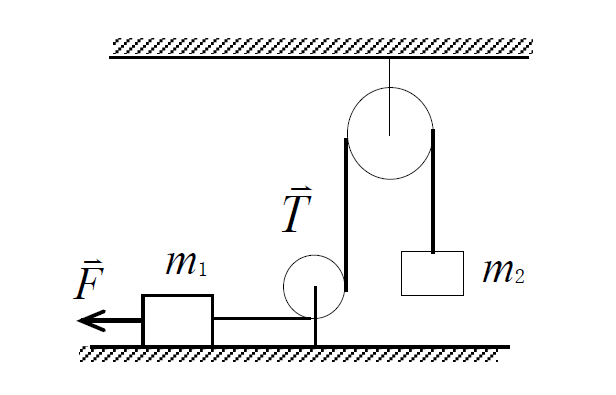
\includegraphics[width=0.15\textheight]{fig5}
        \caption{如图}\label{Fig:5}
    \end{figure}

\end{enumerate}

\subsection*{二、选择题}
\begin{enumerate}
\item 如图 \ref{Fig:6} , 在$m_A>μm_B$的条件下,可算出$m_B$向右运动的加速度$a$,今如取去$m_A$而代之以拉力$T=m_Ag$,算出的加速度$a′$则有: ( C )
\twoch{$a>a^{'}$ }{$a=a^{'}$ }{$a<a^{'}$ }{不能确定}
    \begin{figure}[H]
        \centering
        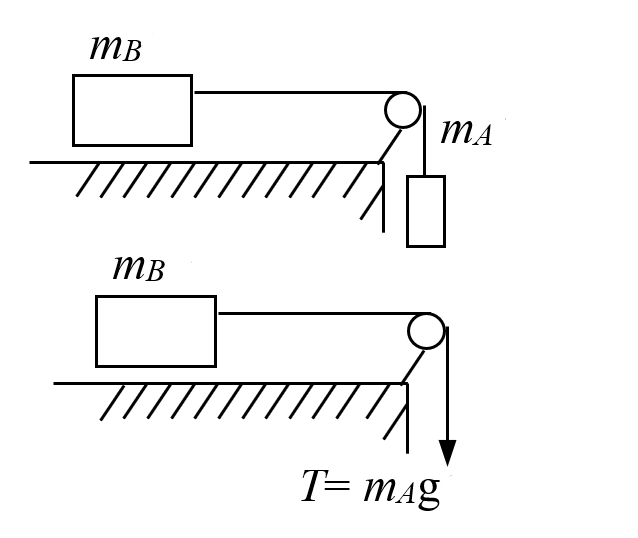
\includegraphics[width=0.15\textheight]{fig6}
        \caption{如图}\label{Fig:6}
    \end{figure}
    \begin{note}
        \textcolor{red}{
        摩擦力$f = \mu m_B g$, 情况一: $m_Ag - f = (m_A + m_B)a$, 情况二: $m_Ag - f = m_B a{'}$.}
    \end{note}
\item 如图\ref{Fig:7} , $m$与$M$,$M$与水平桌面间都是光滑接触,为维持$m$与$M$相对静止,则推动$M$的水平力$F$为( B )
\twoch{$(m+M)g\mathrm{cot}\theta$}{$(m+M)g\mathrm{tan}\theta$}{$mg\mathrm{tan}\theta$}{$Mg\mathrm{tan}\theta$}.
    \begin{figure}[H]
        \centering
        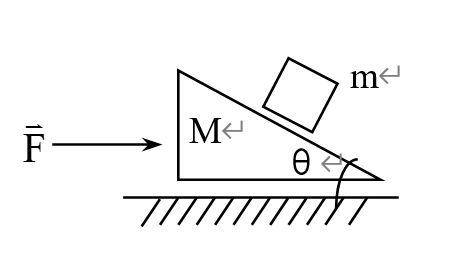
\includegraphics[width=0.15\textheight]{fig7}
        \caption{如图}\label{Fig:7}
    \end{figure}
    \begin{note}
        看图, 懒得自己写了(其实自己写得不咋样):
    \end{note}
    \begin{figure}[H]
        \centering
        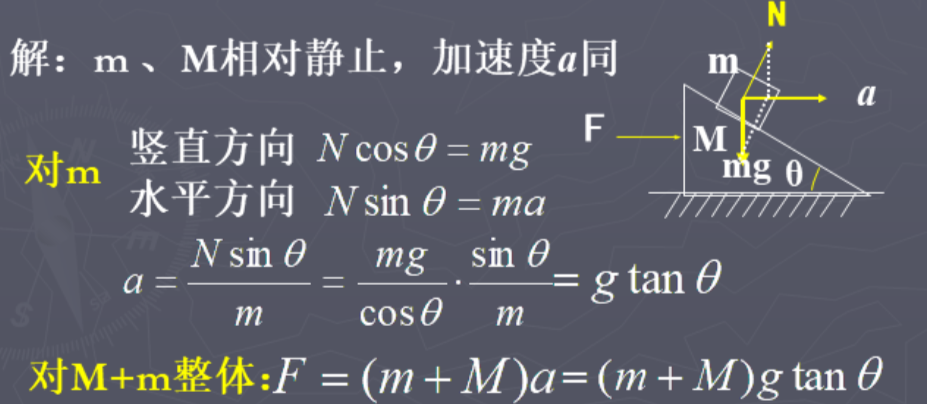
\includegraphics[width=0.25\textheight]{ans2}
    \end{figure}
\item 一质量为$m$的质点, 自半径为$R$的光滑半球形碗口由静止下滑, 质点在碗内某处的速率为$V$, 则质点对该处的压力数值为( B )
\twoch{$\frac{mV^2}{R}$}{$\frac{3Mv^2}{2R}$}{$\frac{2mV^2}{R}$}{$\frac{5mV^2}{2R}$}
\begin{note}
    看图, 懒得自己写了(其实自己写得不咋样):
\end{note}
\begin{figure}[H]
    \centering
    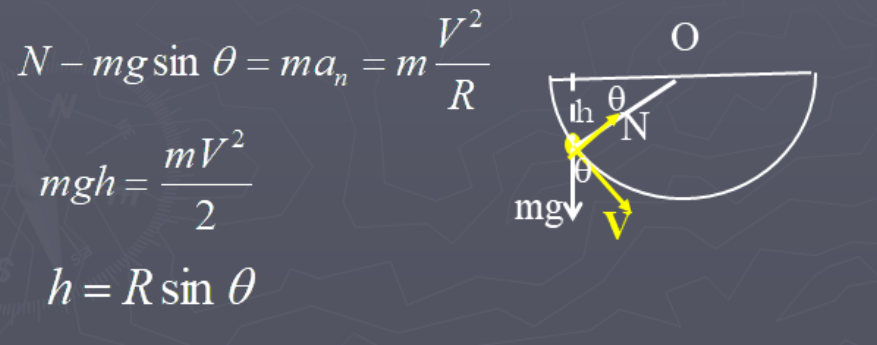
\includegraphics[width=0.25\textheight]{ans1}
\end{figure}
\item 如图 \ref{Fig:8} ,滑轮、绳子质量及运动中的摩擦阻力都忽略不计,物体$A$的质量$m_1$大于物体B的质量$m_2$.在$A$、$B$运动过程中弹簧秤$S$的读数是( D )
\twoch{$(m_1+m_2)g$}{$(m_1-m_2)g$}{$\frac{2m_1m_2}{m_1+m_2}g$}{$\frac{4m_1m_2}{m_1+m_2}g$}
    \begin{figure}[H]
        \centering
        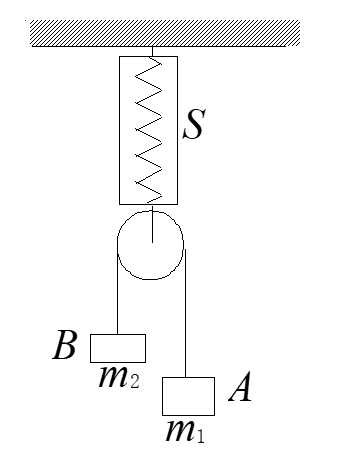
\includegraphics[width=0.15\textheight]{fig8}
        \caption{如图}\label{Fig:8}
    \end{figure}

\begin{note}
    \textcolor{red}{先受力分析, 再计算}
    \begin{figure}[ht]
        \begin{minipage}[ht]{0.6\linewidth}
            \begin{table}[H]
                \begin{tabular}{l}
                   \qquad 计算过程:\\
                   \qquad \qquad $m_1g-T=m_1a, T-m_2g = m_2a$ \\
                    \qquad \qquad   $\Longrightarrow T = \frac{2m_1m_2}{m_1+m_2}g$ \\
                    \qquad \qquad $\Longrightarrow F = 2T =\frac{4m_1m_2}{m_1+m_2}g$\\ 
                \end{tabular}
            \end{table}  
        \end{minipage}
        \begin{minipage}[H]{0.3\linewidth}
            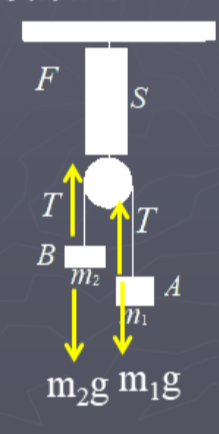
\includegraphics[width=0.08\textheight]{ans3}
        \end{minipage}
    \end{figure}
\end{note}
\item 如图所示 \ref{Fig:9},质量为$m$的物体$A$用平行于斜面的细线连结置于光滑的斜面上,若斜面向左方作加速运动,当物体开始脱离斜面时,它的加速度的大小为( C )
\twoch{$g\mathrm{sin}\theta$}{$g\mathrm{cos}\theta$}{$g\mathrm{cot}\theta$}{$g\mathrm{tan}\theta$}
    \begin{figure}[H]
        \centering
        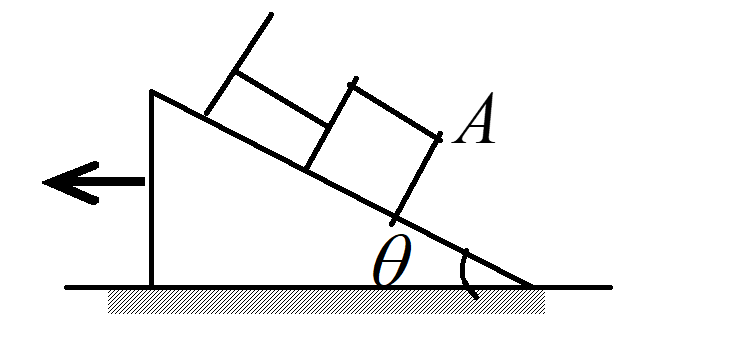
\includegraphics[width=0.15\textheight]{fig9}
        \caption{如图}\label{Fig:9}
    \end{figure}
    \begin{note}
        \textcolor{red}{临界运动状态斜面对物体支持力为零}
        \begin{figure}[ht]
            \begin{minipage}[ht]{0.6\linewidth}
                \begin{table}[H]
                    \begin{tabular}{l}
                       \qquad 计算过程:\\
                       \qquad \qquad $T \mathrm{cos}\theta=ma$ \\
                       \qquad \qquad $T \mathrm{sin}\theta=mg$ \\
                    \end{tabular}
                \end{table}  
            \end{minipage}
            \begin{minipage}[H]{0.3\linewidth}
                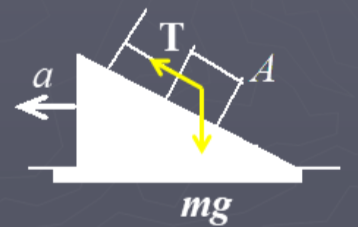
\includegraphics[width=0.15\textheight]{ans4}
            \end{minipage}
        \end{figure}
    \end{note}
\item 站在电梯内的一个人, 看到用细线连结的质量不同的两个物体跨过电梯内的一个无摩擦的定滑轮而处于“平衡”状态. 由此, 他断定电梯作加速运动, 其加速度为( B )
\twoch{大小为$g$, 方向向上}{大小为$g$, 方向向下}{大小为$\frac{1}{2}g$,方向向上}{大小为$\frac{1}{2}g$, 方向向下}
\begin{note}
    \textcolor{red}{由“平衡”状态得出绳子$T=0$}
    \begin{figure}[ht]
        \begin{minipage}[ht]{0.6\linewidth}
            \begin{table}[H]
                \begin{tabular}{l}
                   \qquad 计算过程:\\
                   \qquad \qquad $m_1 g = m_1a$ \\
                   \qquad \qquad $m_2 g = m_2a$ \\
                \end{tabular}
            \end{table}  
        \end{minipage}
        \begin{minipage}[H]{0.3\linewidth}
            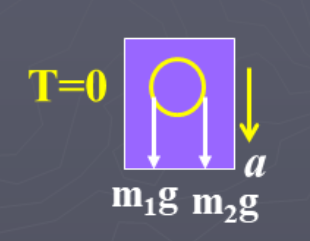
\includegraphics[width=0.15\textheight]{ans5}
        \end{minipage}
    \end{figure}
\end{note}
\end{enumerate}


\subsection*{三、计算题}
\begin{enumerate}
    \item 如图 \ref{Fig:10} , 已知$m_A=2kg, m_B=1kg, m_A, m_B$与桌面间的摩擦系数$\mu=0.5(g=10m/s^2)$
    \begin{enumerate}
    \item[(1)] 今用水平力$F=10N$推$m_B$, 求$m_A$与$m_B$的摩擦力$f$及$m_A$的加速度$a_A$ ;
    \item[(2)] 今用水平力$F=20N$推$m_B$, 求$m_A$与$m_B$的摩擦力$f$及$m_A$的加速度$a_A$ .
        \begin{figure}[H]
            \centering
            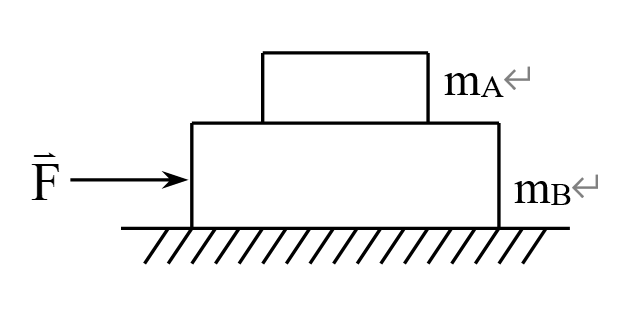
\includegraphics[width=0.15\textheight]{fig10}
            \caption{如图}\label{Fig:10}
        \end{figure}
    \end{enumerate}
    \begin{solution}
        \begin{enumerate}
           \item[(1)]   $F<u(m_A+m_B)g=15N$  $\therefore$ A、B无相对运动  $\therefore f=0,a_A=0$
           \item[(2)]     看图: 
         
           \begin{figure}[H]
               \centering
               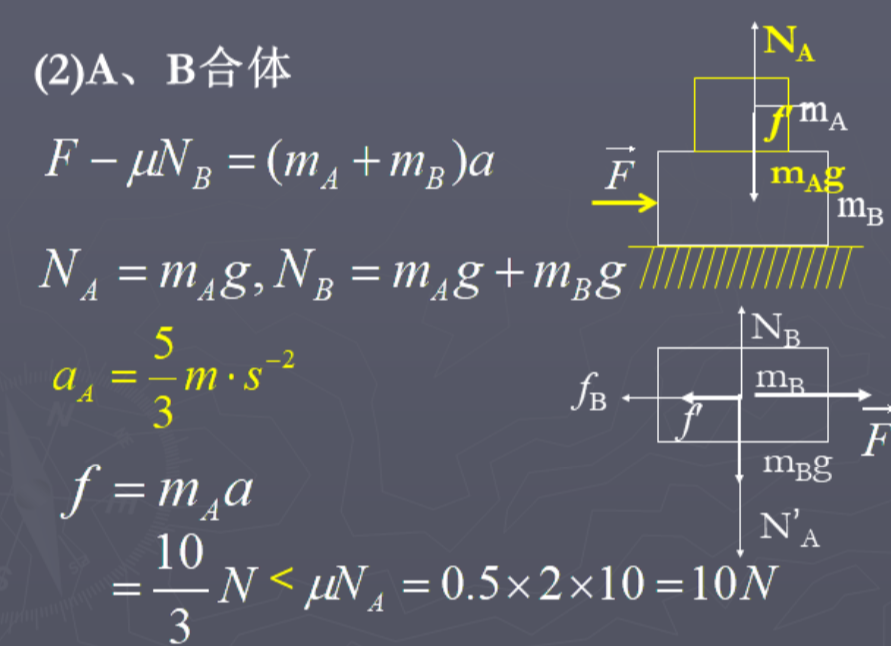
\includegraphics[width=0.5\textheight]{ans6}
           \end{figure}
        \end{enumerate}
        
    \end{solution}
    \item 如图 \ref{Fig:11} , 光滑水平面上平放着半径为$R$的固定环,环内的一物体以速率$V_0$开始沿环内侧逆时针方向运动,物体与环内侧的摩擦系数为$\mu$, 求:
    \begin{enumerate}
        \item[(1)] 物体任一时刻$t$的速率$V$;                                            
        \item[(2)] 物体从开始运动经$t$秒经历的路程$S$.
        \begin{figure}[H]
            \centering
            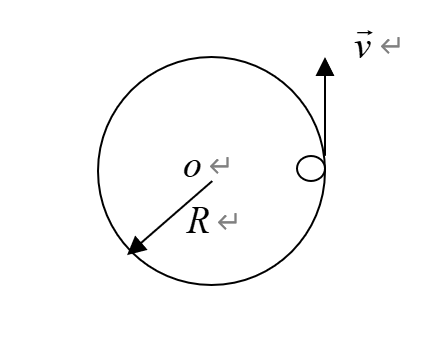
\includegraphics[width=0.15\textheight]{fig11}
            \caption{如图}\label{Fig:11}
        \end{figure} 
    \end{enumerate}
    \begin{solution}
        受力分析图如下:
        \begin{figure}[H]
            \centering
            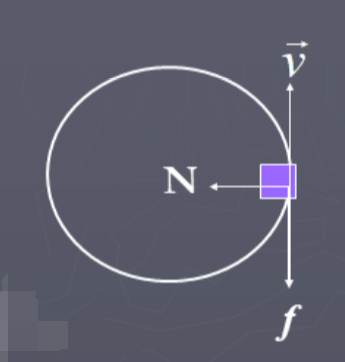
\includegraphics[width=0.15\textheight]{ans7}
        \end{figure} 
        \begin{enumerate}
            \item[(1)]对物体受力分析, 得出$\begin{cases}
                -f = m\frac{\mathrm{d}v}{\mathrm{d}t} \\
                N = m\frac{v^2}{R}\\
                f = \mu N
            \end{cases}$ \ \ $\therefore -\mu \frac{v^2}{R} = \frac{\mathrm{d}v}{\mathrm{d}t}$, 对两边积分得\\ 
            $\displaystyle{\int_{v_0}^{v} \frac{\mathrm{d}v}{v^2}}=\int_0^t -u \frac{\mathrm{d}t}{R}$, $\frac{1}{v_0}-\frac{1}{v}=-\frac{\mu}{R}t$
            $\therefore v = \frac{v_0R}{R+v_0 \mu t}$
            \item[(2)] $\frac{\mathrm{d}s}{\mathrm{d}t}=v=\frac{v_0R}{R+v_0\mu t}$\ \ 
            $\therefore s = \displaystyle{\int_0^t \frac{v_0 R\mathrm{d}t}{R+v_0\mu t}=\frac{R}{\mu}\mathrm{ln}(1+\frac{v_0\mu t}{R})}$. 
        \end{enumerate}
    \end{solution}
\end{enumerate}
